\documentclass[11pt,a4paper,english]{article}

% Code with metapost output thanks to YannD at texnique.fr
% https://texnique.fr/osqa/questions/11076/comment-obtenir-le-code-metapost-et-la-figure-dans-un-document-avec-luamplib

% To compile:
% lualatex repere-doc.tex

  \usepackage{mathtools}
\usepackage{unicode-math}
\setmainfont{STIX Two Text}
\setmathfont{STIX Two Math}
\usepackage{fontawesome5}

\usepackage{geometry}
\geometry{hmargin=2cm,vmargin={1.5cm,1.8cm},includefoot}

  \usepackage[bottom]{footmisc}

  \usepackage{mflogo}

  \usepackage[output-decimal-marker={,}]{siunitx}
  \usepackage{esvect}
  \usepackage{nicefrac}

  \usepackage{multicol}
  \setlength{\multicolsep}{3pt}
  \setlength{\columnsep}{0pt}

  \usepackage[toc]{multitoc}

  \usepackage{enumitem}

  \usepackage[svgnames]{xcolor}

  \usepackage{graphicx}

  \usepackage{url}
  \usepackage{verbatim}
  \usepackage{fancyvrb}

  \usepackage{array}
  \usepackage{colortbl}
  \usepackage{tabularx}
  \renewcommand{\tabularxcolumn}[1]{>{\arraybackslash}m{#1}}
  \newcolumntype{M}[1]{>{\arraybackslash}m{#1}}
  \usepackage{longtable}
  \usepackage{tabularray}

\usepackage{luamplib}
\everymplib{verbatimtex \leavevmode etex;
            input mptrees;
            beginfig(1);}
\everyendmplib{endfig;}
\mplibnumbersystem{decimal}

\usepackage{tcolorbox}
\tcbuselibrary{listings,skins}%,documentation}

  \usepackage{babel}


\usepackage{marginnote}

\usepackage[colorlinks=true,urlcolor=blue]{hyperref}
%\hypersetup{colorlinks=true,allcolors=red,linkcolor=red}

\usepackage{listings}

  \lstset{columns=flexible,%
          basicstyle=\color{darkgray}\ttfamily,
          literate={é}{{\'e}}1,
          keywordstyle=\color{black}\bfseries}

\lstdefinestyle{mpost}{language={MetaPost},
                       morekeywords={tree}
                       }

\makeatletter
\tcbset{%
    listing metapost/.code={%
        \def\tcbuselistingtext@input{%
                   \begin{mplibcode}
                       input \jobname.listing;
                   \end{mplibcode}}%
    }
}
\makeatother

\definecolor{CoulParam}{rgb}{0.4,0,0.5}

\definecolor{TestC}{rgb}{0.963,0.971,0.994}
\colorlet{FondCommandes}{black!60!yellow!10!white}

\tcbset{boites/.style={left=1em,right=1em,
                       colback=white,
                       boxrule=0pt,
                       colframe=white,
                       fonttitle=\bfseries\ttfamily,
                       colbacktitle=FondCommandes,
                       before title={\hspace{-1em}},
                       arc=0pt,
                       after=\medskip,
                      }}

\DeclareTColorBox{rpobjet}{ v m }{
           boites,
           title={#1},
           coltitle=blue,
           colbacktitle=blue!5!white,
           after title={\hfill #2},
           }

\DeclareTColorBox{mptparam}{ v m v}{
           boites,
           title={#1},
           coltitle=CoulParam,
           colbacktitle=CoulParam!5!white,
           after title={\hfill #2, {\normalfont default :} #3},
           }

\DeclareTColorBox{rpdeclaration}{ v }{
           boites,
           title={#1},
           coltitle=black,
           colbacktitle=black!5!white,
           }

\DeclareTColorBox{rplabel}{ v }{
           boites,
           title={#1},
           coltitle=red,
           colbacktitle=red!50!black!5!white,
           }

\DefTblrTemplate{contfoot-text}{default}{}
\DefTblrTemplate{conthead-text}{default}{}
\DefTblrTemplate{caption-tag}{default}{}
\DefTblrTemplate{caption-sep}{default}{}
\DefTblrTemplate{caption-text}{default}{}
\NewDocumentEnvironment{rpparam}{ +b}
             {\par\medskip\begin{center}
             \begin{longtblr}[label=none,caption={}]{
             rowhead=2,
             verb,
             hlines={2pt,white},
             columns={c},
             row{1}=white,
             row{2-Z}={bg=CoulParam!5!white,m},
             column{4}={wd=8cm,fg=black,j},
             cell{3-Z}{1-3}={cmd=\testparam},
             cell{3-Z}{1}={cmd=\bfseries\testparam}
             }
             \SetCell[c=4]{c} Paramètres \\
             Nom & Type & Défaut &  \\
             #1
             \end{longtblr}
             \end{center}\bigskip}
             {}



\tcbset{mot/.style={colback=FondCommandes,
        verbatim,
        arc=0pt,
        outer arc=0pt,
        top=0pt,bottom=0pt,left=0mm,right=0mm,
        boxrule=0pt}}

\DeclareTotalTCBox{\rpdec}{v}{mot,coltext=black}{#1}
\DeclareTotalTCBox{\rpfig}{v}{mot,coltext=blue}{#1}
\DeclareTotalTCBox{\rplab}{v}{mot,coltext=red}{#1}
\DeclareTotalTCBox{\rppar}{v}{mot,coltext=CoulParam}{#1}

\NewDocumentCommand{\testparam}{v}{\textcolor{CoulParam}{\texttt{#1}}}
\NewDocumentCommand{\desstab}{v}{\textbf{\texttt{#1}}}

\NewDocumentCommand{\decfig}{m}{\raisebox{-.45\height}{#1}}



\DeclareTCBListing[auto counter]{exemple}{ !O{} }{
    enhanced,
    title=Example \thetcbcounter,
    coltitle=black,
    fonttitle=\bfseries,
    attach boxed title to top left,
    boxed title style={left=0pt,
                       boxrule=0pt,
                       colframe=white,
                       colback=white,
                       coltext=black},
    colback=red!25!yellow!10!white,
    left=1mm,top=0mm,bottom=0mm,
    halign lower=center,
    listing metapost,
    listing outside text,
%    listing only,
    sidebyside gap=1mm,
    after skip=2em,
    before upper={\texttt{beginfig(\thetcbcounter);}\par\vspace{-0.5\baselineskip}},
    after upper={\par\vspace{-0.5\baselineskip}\texttt{endfig;}},
    listing options={style=mpost
                    },
    #1}


\DeclareTCBListing{codelatex}{ !O{} }{
    enhanced,
    notitle,
    colback=LightSteelBlue,
    left=2mm,top=0mm,bottom=0mm,
    listing only,
    listing options={language={[LaTeX]TeX}
                    },
    #1}

\DeclareTCBListing{codempost}{ !O{} }{
    enhanced,
    notitle,
    colback=red!25!yellow!10!white,
    left=2mm,top=0mm,bottom=0mm,
    after skip=1em,
    listing only,
    listing options={style=mpost
                    },
    #1}


\newcommand{\btet}{%
\begin{tcolorbox}[fontupper=\ttfamily,
nobeforeafter,
%tcbox raise base,
arc=0pt,
outer arc=0pt,
width=1.5cm,
top=0pt,bottom=0pt,left=0mm,right=0mm,
leftrule=0pt,rightrule=0pt,toprule=0.3mm,bottomrule=0.3mm,
boxsep=0.5mm,
colback=red!10!white,colframe=red!50!black]
\scriptsize begintree;\par endtree;
\end{tcolorbox}%
}


\begin{document}
\title{Documentation of \texttt{mptrees.mp}}
\date{\today}
\author{Olivier \textsc{Péault}%
\footnote{E-mail : \href{mailto:o.peault@posteo.net}{\texttt{o.peault@posteo.net}}}}
\maketitle

\setcounter{tocdepth}{2}

\setlength{\columnsep}{25pt}
\tableofcontents
\setlength{\columnsep}{10pt}


\newcommand{\ijc}{[i][j]}

\reversemarginpar



\part{Trees}

\section{Overview}

The first aim of this package is to simplify the drawing of probability trees (or other kind of "tree") with \MP. It provides one main command and several parameters to control the output.

It can be used in standalone files with two compilations (\verb|latexmp| package is loaded) but  also  with Lua\LaTeX{} and \verb|luamplib| package.


\begin{rpobjet}{tree[<i>][<j>](<dim1>,<dim2>,...)(<ev1>,<prob1>,<ev2>,<prob2>,...)}{picture}
Probability tree located in column \verb|i| and row \verb|j| (see figure below). \verb|dim1|, \verb|dim2|,... can be numerics or pairs and control the dimension of the tree. \verb|ev1|, \verb|prob1|... can be strings or pictures and will be printed (using \verb|latexmp| if strings) at the end of the edge (the event) and above the edge (the probability).


\end{rpobjet}


\begin{center}
\begin{mplibcode}
draw tree[1][1](3cm,2cm)("$A$","$p$","$\overline{A}$","$q$");
draw tree[2][1](3cm,1cm)("$B$","$\nicefrac{1}{4}$","$\overline{B}$","$\nicefrac{3}{4}$");
draw tree[2][2](3cm,1cm)("$B$","$0.5$","$\overline{B}$","$0.5$");
draw tree[3][2](3cm,1cm)("$C$","$c$","$\overline{C}$","$1-c$");
draw tree[4][2](3cm,1cm)("$D$","$a$","$\overline{D}$","$b$");
drawoptions(dashed evenly);
draw (Orig_arbre[2][1]+(0,0.5cm))--(Orig_arbre[2][2]-(0,0.5cm))--(Orig_arbre[2][2]-(3.5cm,0.5cm))--(Orig_arbre[2][1]+(-3.5cm,0.5cm))--cycle withcolor red;
label.bot(textext("\texttt{tree[1][1]}"),0.5[Orig_arbre[2][2]-(0,0.5cm),Orig_arbre[2][2]-(3.5cm,0.5cm)]) withcolor red;
draw (Orig_arbre[3][1]+(0,0.5cm))--(Orig_arbre[3][2]-(0,0.5cm))--(Orig_arbre[2][1]-(0,1cm))--(Orig_arbre[2][1]+(0,1cm))--cycle withcolor 0.5green;
label.top(textext("\texttt{tree[2][1]}"),0.5[Orig_arbre[3][1]+(0,0.5cm),Orig_arbre[2][1]+(0,1cm)]) withcolor 0.5green;
draw (Orig_arbre[3][3]+(0,0.5cm))--(Orig_arbre[3][4]-(0,0.5cm))--(Orig_arbre[2][2]-(0,1cm))--(Orig_arbre[2][2]+(0,1cm))--cycle withcolor 0.5green;
label.bot(textext("\texttt{tree[2][2]}"),0.5[Orig_arbre[3][4]-(0,0.5cm),Orig_arbre[2][2]-(0,1cm)]) withcolor 0.5green;
draw (Orig_arbre[4][1]+(0,0.5cm))--(Orig_arbre[4][2]-(0,0.5cm))--(Orig_arbre[3][2]-(0,1cm))--(Orig_arbre[3][2]+(0,1cm))--cycle withcolor blue;
label.bot(textext("\texttt{tree[3][2]}"),0.5[Orig_arbre[4][2]-(0,0.5cm),Orig_arbre[3][2]-(0,1cm)]) withcolor blue;
draw (Orig_arbre[5][1]+(0,0.5cm))--(Orig_arbre[5][2]-(0,0.5cm))--(Orig_arbre[4][2]-(0,1cm))--(Orig_arbre[4][2]+(0,1cm))--cycle withcolor red;
label.bot(textext("\texttt{tree[4][2]}"),0.5[Orig_arbre[5][2]-(0,0.5cm),Orig_arbre[4][2]-(0,1cm)]) withcolor red;
\end{mplibcode}

\end{center}


\marginnote[\btet]{}Note that you can use these commands inside any \verb|beginfig();...endfig;| but sometimes, for some constructions, they need to be enclosed between \verb|begintree| and \verb|endtree| commands. Such commands are indicated with a margin note.

\section{Trees}
\subsection{Different kinds of trees}

\begin{rpobjet}{tree[<i>][<j>](<width>,<vspace>)(<ev1>,<prob1>,<ev2>,<prob2>,...)}{picture}
Regular tree where \verb|width| is the horizontal width of the tree and \verb|vspace| the vertical space between two consecutive nodes.
\end{rpobjet}





\mplibcodeinherit{enable}

\begin{mplibcode}
string dim[];dim[4]:="4 cm";dim[3]:="3 cm";dim[2]:="2 cm";dim[1]:="1 cm";dim[15]:="1.5 cm";dim[25]:="2.5 cm";dim[11]:="-1 cm";dim[22]:="-2 cm";dim[7]:="7cm";
\end{mplibcode}

\everyendmplib{drawoptions(withcolor red);drawdblarrow ((0,0)--(4cm,0)) shifted (0,2.25cm);label.top(textext(dim[4]),(2cm,2.25cm));drawdblarrow ((0,0)--(0,2.5cm)) shifted (Orig_arbre[2][2]-(5cm,0));label.lft(textext(dim[25]),(-1cm,0));drawoptions(withcolor 0.5green);drawdblarrow ((0,0)--(3cm,0)) shifted (Orig_arbre[2][1]+(0,1cm));label.top(textext(dim[3]),(6cm,2.25cm));drawdblarrow ((0,0)--(0,1.5cm)) shifted (Orig_arbre[3][2]+(0.25cm,0));label.rt(textext(dim[15]),Orig_arbre[3][2]+(0.25cm,0.75cm));drawdblarrow ((0,0)--(0,1cm)) shifted (Orig_arbre[3][4]+(0.25cm,0));label.rt(textext(dim[1]),Orig_arbre[3][4]+(0.25cm,0.5cm));drawdblarrow ((0,0)--(0,1cm)) shifted (Orig_arbre[3][5]+(0.25cm,0));label.rt(textext(dim[1]),Orig_arbre[3][5]+(0.25cm,0.5cm));endfig;}

\begin{exemple}[listing above text]
draw tree[1][1](4cm,2.5cm)("$A_1$","$\nicefrac{1}{3}$","$A_2$","$\nicefrac{2}{3}$");
draw tree[2][1](3cm,1.5cm)("$B$","$\nicefrac{1}{4}$","$C$","$\nicefrac{3}{4}$");
draw tree[2][2](3cm,1cm)("$D$","$p$","$E$","$q$","$F$","$r$");
\end{exemple}

\begin{rpobjet}{tree[<i>][<j>](<width>,<vsp1>,<vsp2>,...)(<ev1>,<p1>,<ev2>,<p2>,...)}{picture}
Tree where \verb|width| is the horizontal width of the tree while each \verb|vsp| indicates the vertical space between the node and the origin of the tree.

\end{rpobjet}

\everyendmplib{
drawoptions(withcolor 0.5green);
draw Orig_arbre[2][1] -- (Orig_arbre[2][1]+(4.5cm,0)) dashed evenly;
drawdblarrow ((0,0)--(3cm,0)) shifted (Orig_arbre[2][1]+(0,2.25cm));label.top(textext(dim[3]),(5cm,3.25cm));
drawarrow ((0,-2cm)--(0,0)) shifted (Orig_arbre[3][1]+(0.25cm,0));label.rt(textext(dim[2]),Orig_arbre[3][1]+(0.25cm,-0.7cm));
drawarrow ((0,-1cm)--(0,0)) shifted (Orig_arbre[3][2]+(0.5cm,0));label.rt(textext(dim[1]),Orig_arbre[3][2]+(0.5cm,-0.5cm));
drawarrow ((0,1cm)--(0,0)) shifted (Orig_arbre[3][3]+(0.75cm,0));label.rt(textext(dim[11]),Orig_arbre[3][3]+(0.75cm,0.5cm));
drawarrow ((0,0)--(0,-2cm)) shifted (Orig_arbre[3][4]+(0.25cm,0));label.rt(textext(dim[22]),Orig_arbre[3][4]+(0.25cm,-1cm));
endfig;}

\begin{exemple}[listing above text]
draw tree[1][1](3cm,2cm)("$A$","$p$","$\overline{A}$","$q$");
draw tree[2][1](3cm,2cm,1cm,-1cm)("$B$","$p$","$C$","$q$","$D$","$r$");
draw tree[2][2](3cm,0cm,-2cm)("$E$","$0.5$","$F$","$0.5$");
\end{exemple}


\begin{rpobjet}{tree[<i>][<j>](<pair1>,<pair2>,...)(<ev1>,<prob1>,<ev2>,<prob2>,...)}{picture}
Tree where \verb|pair1|, \verb|pair2|... indicate the coordinates of each node from the origin of the tree.
\end{rpobjet}

\everyendmplib{
drawoptions(withcolor 0.5green);
draw Orig_arbre[2][1] -- (Orig_arbre[2][1]+(5cm,0)) dashed evenly;
drawarrow ((0,0)--(3cm,0)) shifted (Orig_arbre[2][1]+(0,2.25cm));label.top(textext(dim[3]),(5cm,3.25cm));
drawarrow ((0,-2cm)--(0,0)) shifted (Orig_arbre[3][1]+(0.25cm,0));label.rt(textext(dim[2]),Orig_arbre[3][1]+(0.25cm,-0.7cm));
drawarrow ((0,0)--(4cm,0)) shifted (Orig_arbre[2][1]+(0,-1.25cm));label.bot(textext(dim[4]),(5.5cm,-0.25cm));
drawarrow ((0,0)--(0,-1cm)) shifted (Orig_arbre[3][2]+(0,1cm));label.rt(textext(dim[11]),Orig_arbre[3][2]+(0,0.5cm));
endfig;}

\begin{exemple}[listing above text]
draw tree[1][1](3cm,2cm)("$A$","$p$","$\overline{A}$","$1-p$");
draw tree[2][1]((3cm,2cm),(4cm,-1cm))("$B$","$q$","$C$","$r$");
\end{exemple}

\everyendmplib{endfig;}


\subsection{Simple trees}
\begin{rpobjet}{stree[<i>][<j>](...)(<ev1>,<ev2>)}{picture}
Same as previous except that there are no probabilities.
\end{rpobjet}


\begin{exemple}[listing above text]
draw stree[1][1](100,50)("$A$","$B$","$C$");
draw stree[2][1](80,25)("$A$","$B$");
draw stree[2][2](80,25)("$A$","$B$");
draw stree[2][3](80,25)("$A$","$B$");
\end{exemple}

\subsection{Start and end labels}
\begin{rpobjet}{startlabel(<s>)}{picture}
Prints \verb|s| (can be a string or a picture) at the origin of the tree.
\end{rpobjet}


\begin{exemple}[lefthand ratio = 0.65]
 draw startlabel("$S$");
 draw tree[1][1](3cm,2cm)("$A$","$p$","$B$","$q$");
\end{exemple}

\begin{rpobjet}{endlabel[<i>][<j>](<s>)}{picture}
Prints \verb|s| at the end of a branch. The space between the previous label ans \verb|s| is controlled by the numeric \verb|endlabelspace| which defaults to \verb|1cm|.
\end{rpobjet}

\begin{exemple}[listing above text]
 draw startlabel("$S$");
 draw tree[1][1](3cm,2cm)("$A$","$p$","$B$","$q$");
 draw tree[2][2](2cm,1cm)("$A$","$p$","$B$","$q$");
 draw endlabel[2][1]("$SA$");
 draw endlabel[3][1]("$SBA$");
 draw endlabel[3][2]("$SBB$");
\end{exemple}

\section{Direction}

\begin{mptparam}{dirtree}{numeric}{0}
All trees are construct horizontally by default. \verb|ditree| indicates the angle in degrees between the horizontal and the main direction of the tree.
\end{mptparam}

\begin{exemple}[listing above text]
dirtree:=135;
draw tree[1][1](3cm,2cm)("$A_1$","$a_1$","$A_2$","$a_2$");
draw tree[2][1](3cm,1cm)("$B$","$b$","$C$","$c$");
draw tree[2][2](3cm,1cm)("$D$","$p$","$E$","$q$");
\end{exemple}


\begin{exemple}[listing above text]
dirtree:=-60;
draw tree[1][1](3cm,2cm)("$A_1$","$a_1$","$A_2$","$a_2$");
draw tree[2][1](3cm,1cm)("$B$","$b$","$C$","$c$");
draw tree[2][2](3cm,1cm)("$D$","$p$","$E$","$q$");
\end{exemple}


\begin{mptparam}{dirlabel}{numeric}{0}
All the trees are viewed as ``horizontal" trees, so the space between two subtrees is horizontal too. With \verb|dirtree|, the whole (horizontal) tree is rotated. But if the tree is designed vertically, spacing is wrong. In this case, one can use \verb|dirlabel| to indicate the orientation of the tree.
\end{mptparam}


\begin{exemple}[lefthand ratio=0.65]
draw tree[1][1]((-1cm,2cm),(1cm,2cm))
                              ("$A$","$p$","$B$","$q$");
draw tree[2][1]((-0.5cm,2cm),(0.5cm,2cm))
                              ("$C$","$c$","$D$","$d$");
draw tree[2][2]((-0.5cm,2cm),(0.5cm,2cm))
                              ("$E$","$e$","$F$","$f$");
\end{exemple}

\begin{exemple}[lefthand ratio=0.65]
dirlabel:=90;
draw tree[1][1]((-1cm,2cm),(1cm,2cm))
                              ("$A$","$p$","$B$","$q$");
draw tree[2][1]((-0.5cm,2cm),(0.5cm,2cm))
                              ("$C$","$c$","$D$","$d$");
draw tree[2][2]((-0.5cm,2cm),(0.5cm,2cm))
                              ("$E$","$e$","$F$","$f$");
\end{exemple}

\section{Dealing with alignment}

\begin{mptparam}{shiftev}{numeric}{-1}
The origin of each tree is located at the right side of the bounding box of the previous event name. Thus different subtrees may begin at different places. The numeric \verb|shiftev|, if positive, indicates the fixed horizontal space between the end of the edges and the beginning of following subtrees.

It can be used inside the first set of parameters of the tree (see example below) or as a global variable.
\end{mptparam}

\begin{exemple}[listing above text]
 draw tree[1][1](80,120)("$A$","$0.5$","$\overline{A}$","$0.5$");
 draw tree[2][1](70,40)("Yes","$p$","No","$q$","Maybe","$r$");
 draw tree[2][2](70,40,"shiftev:=1.5cm")("Yes","$p$","No","$q$","Maybe","$r$");
 draw tree[3][1](50,20)("$B$","$b$","$C$","$c$");
 draw tree[3][2](50,20)("$B$","$b$","$C$","$c$");
 draw tree[3][3](50,20)("$B$","$b$","$C$","$c$");
 draw tree[3][4](50,20)("$B$","$b$","$C$","$c$");
 draw tree[3][5](50,20)("$B$","$b$","$C$","$c$");
 draw tree[3][6](50,20)("$B$","$b$","$C$","$c$");
\end{exemple}

\begin{mptparam}{abscoord}{boolean}{false}
With the boolean \verb|abscoord| set to \verb|true|, all the coordinates are given from the origin of the \emph{first} tree instead of the origin of the subtree, which makes easier the alignment of all the subtrees.
\end{mptparam}


\everyendmplib{drawoptions(withcolor red);
drawdblarrow ((0,0)--(7cm,0)) shifted (0,2cm);label.top(textext(dim[7]),(3.5cm,2cm));
drawdblarrow ((0,0)--(0,1.5cm)) shifted (-0.5cm,0);label.lft(textext("1.5 cm"),(-0.5cm,0.75cm));
endfig;}

\begin{exemple}[listing above text]
abscoord:=true;
draw tree[1][1](3cm,2cm)("$A$","$p$","Blabla","$q$");
draw tree[2][1]((7cm,1.5cm),(7cm,0.5cm))("$A$","$p$","$B$","$q$");
draw tree[2][2]((7cm,-0.5cm),(7cm,-1.5cm))("$A$","$p$","$B$","$q$");
\end{exemple}

\everyendmplib{endfig;}

\section{Parameters}

All following parameters can be changed globally before drawing the tree or changed locally inside the first set of parameters:

\begin{codempost}[width=0.7\linewidth,left skip=1cm]
scaleev:=2;
draw tree[1][1](3cm,2cm)(...);
draw tree[2][1](3cm,2cm)(...);
\end{codempost}

or

\begin{codempost}[width=0.7\linewidth,left skip=1cm]
draw tree[1][1](3cm,2cm,"scaleev:=2")(...);
draw tree[2][1](3cm,2cm)(...);
\end{codempost}

In the fisrt case, \verb|scaleev| is changed globally while in the second case, the change only applies to the first tree.


\subsection{Event}

\begin{mptparam}{scaleev}{numeric}{1}
Numeric controlling the scale of the label at the end of the edge (the event).
\end{mptparam}


\begin{exemple}[lefthand ratio=0.65]
 scaleev:=2;
 draw stree[1][1](3cm,2cm)("$A$","$B$");
\end{exemple}

\begin{mptparam}{nodeformat}{string}{""}
String that indicates how the events are printed (the shape of path around the event). Possible values are (for now) \verb|"bbox"|, \verb|"circle"|, \verb|"superellipse"|.

See below for personalised values.
\end{mptparam}

\begin{exemple}[lefthand ratio=0.65]
 nodeformat:="bbox";
 draw stree[1][1](3cm,2cm)("$A$","$B$");
\end{exemple}

\begin{mptparam}{nodelinecolor}{color}{black}
Color of the path around the node
\end{mptparam}

\begin{mptparam}{nodebgcolor}{color}{white}
Color of the background of the region delimited by the previous path.
\end{mptparam}

\begin{mptparam}{nodefgcolor}{color}{black}
Color of the text.
\end{mptparam}



\begin{exemple}[lefthand ratio=0.65]
nodeformat:="superellipse";
nodelinecolor:=(0.8,0,0);
nodebgcolor:=(1,0.5,0.5);
nodefgcolor:=white;
draw stree[1][1](3cm,2cm)("$A$","$B$");
\end{exemple}


\begin{exemple}[lefthand ratio=0.65]
nodefgcolor:=(0.7,0.4,0.7);
draw stree[1][1](3cm,2cm)("$A$","$B$");
\end{exemple}

\begin{rpobjet}{nodeshape(expr A,B)}{cycle path}
It is also possible to redefine the path defining the node. Simply rewrite the \verb|nodeshape| macro, which must take a picture as parameter and whose result must be a cycle path.

The parameter passed to the macro is the figure representing the drawing of the event (normally the name of the event). You may use it, or not, in the macro definition.
\end{rpobjet}

\begin{exemple}[lefthand ratio=0.6]
vardef nodeshape(expr p)=
  fullcircle xscaled 1cm yscaled 0.6cm
enddef;

draw stree[1][1](3cm,3cm)("$A$","$B$");
\end{exemple}


\begin{exemple}[lefthand ratio=0.7]
vardef nodeshape(expr p)=
  llcorner p..ulcorner p..urcorner p..lrcorner p--cycle
enddef;

nodebgcolor:=0.7white;
draw stree[1][1](3cm,3cm)("$A$","$B$");
\end{exemple}



\subsection{Leaves}
\marginnote[\btet]{}
You may want to format the leaves in a different way from the nodes. A tree using the following parameters must be enclosed in a \verb|begintree;|...\verb|endtree;| ``environment".

\begin{mptparam}{leaveformat}{string}{""}
String that indicates how the events are printed (the shape of path around the event). Possible values are (for now) \verb|"bbox"|, \verb|"circle"|, \verb|"superellipse"| and \verb|"none"|.
\end{mptparam}

\begin{exemple}[listing above text]
begintree;
leaveformat:="bbox";
draw stree[1][1](100,45)("$A$","$B$");
draw stree[2][1](80,30)("$C$","$D$");
draw stree[3][2](65,20)("$E$","$F$");
endtree;
\end{exemple}

\begin{mptparam}{leavelinecolor}{color}{black}
Color of the path around the leave
\end{mptparam}

\begin{mptparam}{leavebgcolor}{color}{white}
Color of the background of the region delimited by the previous path.
\end{mptparam}

\begin{mptparam}{leavefgcolor}{color}{black}
Color of the text.
\end{mptparam}

\begin{exemple}[listing above text]
begintree;
nodeformat:="circle";
nodelinecolor:=(0.8,0,0); nodebgcolor:=(1,0.5,0.5); nodefgcolor:=white;
leaveformat:="bbox";
leavebgcolor:=(0.3,1,1); leavefgcolor:=red;
draw stree[1][1](100,45)("$A$","$B$");
draw stree[2][1](80,30)("$C$","$D$");
draw stree[3][2](65,20)("$E$","$F$");
endtree;
\end{exemple}

Note that \verb|nodeformat| applies to both nodes and leaves. To avoid formatting the leaves, use the value \verb|"none"| for \verb|leaveformat|.

\begin{exemple}[listing above text]
begintree;
nodeformat:="circle";
nodelinecolor:=(0.8,0,0); nodebgcolor:=(1,0.5,0.5); nodefgcolor:=white;
leaveformat:="none";
draw stree[1][1](100,45)("$A$","$B$");
draw stree[2][1](80,30)("$C$","$D$");
draw stree[3][2](65,20)("$E$","$F$");
endtree;
\end{exemple}

\subsection{Probability}

\begin{mptparam}{probformat}{string}{""}
String that indicates how the probabilities are printed (the shape of path around the probability). Possible values are (for now) \verb|"bbox"|, \verb|"circle"|, \verb|"superellipse"|.
\end{mptparam}

\begin{exemple}[lefthand ratio=0.65]
 probformat:="bbox";
 draw tree[1][1](3cm,2cm)("$A$","$p$","$B$","$q$");
\end{exemple}

\begin{mptparam}{problinecolor}{color}{black}
Color of the path around the probability
\end{mptparam}

\begin{mptparam}{probbgcolor}{color}{white}
Color of the background of the region delimited by the previous path.
\end{mptparam}

\begin{mptparam}{probfgcolor}{color}{black}
Color of the text.
\end{mptparam}


\begin{exemple}[lefthand ratio=0.65]
probformat:="circle";
problinecolor:=(0.8,0,0);
probbgcolor:=(1,0.5,0.5);
probfgcolor:=white;
draw tree[1][1](3cm,2cm)("$A$","$p$","$B$","$q$");
\end{exemple}

\begin{exemple}[lefthand ratio=0.65]
probfgcolor:=blue;
draw tree[1][1](3cm,2cm)("$A$","$p$","$B$","$q$");
\end{exemple}


\begin{mptparam}{scaleprob}{numeric}{0.85}
Numeric controlling the scale of the label above the edge (the probability).
\end{mptparam}

\begin{exemple}[lefthand ratio=0.65]
 scaleprob:=1.5;
 draw tree[1][1](3cm,2cm)("$A$","$p$","$B$","$q$");
\end{exemple}


\begin{mptparam}{posprob}{numeric}{0.6}
Numeric controlling the position of the label above the edge.
\end{mptparam}

\begin{exemple}[lefthand ratio=0.65]
 posprob:=0.8;
 draw tree[1][1](3cm,2cm)("$A$","$p$","$B$","$q$");
\end{exemple}


\begin{mptparam}{typeprob}{numeric}{1}
Numeric controlling how the label is printed. Values can be 1 (the label is printed above the edge), 2 (the label is printed on the edge), 3 (the label is printed above the edge and rotated) or 4 (the label is printed on the edge and rotated).
\end{mptparam}

\begin{exemple}[lefthand ratio=0.7]
 typeprob:=2;
 draw tree[1][1](3cm,2cm)("$A$","$p$","$B$","$1-p$");
\end{exemple}

\begin{exemple}[lefthand ratio=0.7]
 typeprob:=3;
 draw tree[1][1](3cm,2cm)("$A$","$p$","$B$","$1-p$");
\end{exemple}

\begin{exemple}[lefthand ratio=0.7]
 typeprob:=4;
 draw tree[1][1](3cm,2cm)("$A$","$p$","$B$","$1-p$");
\end{exemple}



\begin{mptparam}{proboffset}{numeric}{3bp}
Numeric controlling the amount by which the label above the edge is offset.
\end{mptparam}

\begin{exemple}[lefthand ratio=0.75]
 draw tree[1][1](3cm,3cm)("$A$","$p+q+r$","$B$","$s$");
\end{exemple}



\begin{exemple}[lefthand ratio=0.75]
 proboffset:=6bp;
 draw tree[1][1](3cm,3cm)("$A$","$p+q+r$","$B$","$s$");
\end{exemple}


\subsection{Edge}
\begin{mptparam}{linewidth}{numeric}{0.5bp}
Width of the lines.
\end{mptparam}

\begin{mptparam}{linecolor}{color}{black}
Color of the lines.
\end{mptparam}

\begin{exemple}[lefthand ratio=0.65]
 linewidth:=1.5;
 linecolor:=blue;
 draw tree[1][1](3cm,2cm)("$A$","$p$","$B$","$q$");
\end{exemple}

\begin{mptparam}{endedgeshift}{numeric}{0}
Vertical space added at the end of the edge. Useful when various edges end at the same point.
\end{mptparam}

\begin{exemple}[lefthand ratio=0.65]
 draw startlabel("$S$");
 draw tree[1][1]((3cm,-1cm))("$A$","$p$");
\end{exemple}


\begin{exemple}[lefthand ratio=0.65]
 endedgeshift:=10;
 draw startlabel("$S$");
 draw tree[1][1]((3cm,-1cm))("$A$","$p$");
\end{exemple}

\begin{mptparam}{edgearrow}{boolean}{false}
When the boolean \verb|edgearrow| is set to true, edges end with an arrow.
\end{mptparam}

\begin{exemple}[lefthand ratio=0.65]
 edgearrow:=true;
 draw tree[1][1](3cm,2cm)("$A$","$p$","$B$","$q$");
\end{exemple}

\begin{mptparam}{branchtype}{string}{"segment"}
String which indicates the shape of the edge. Possible values are  \verb|segment|, \verb|curve|, \verb|broken|.

Note that double quotes have to be replaced by single quotes when this parameter is changed locally inside the \verb|tree| macro.


See below for personalised values.

\end{mptparam}


\begin{mptparam}{tenscurve}{numeric}{0}
 If string \verb|branchtype| is set to \verb|curve|, \verb|tenscurve| indicates the ``tension". When sets to \verb|1|, the curve is a segment.
 \end{mptparam}

\begin{exemple}[lefthand ratio=0.6]
 branchtype:="curve";
 draw stree[1][1](3cm,3cm)("$A$","$B$");
\end{exemple}


\begin{exemple}[lefthand ratio=0.6]
 draw stree[1][1](3cm,3cm,"branchtype:='curve'")
                                         ("$A$","$B$");
\end{exemple}



\begin{exemple}[lefthand ratio=0.6]
 branchtype:="curve";
 tenscurve:=0.5;
 draw stree[1][1](3cm,3cm)("$A$","$B$");
\end{exemple}


\begin{mptparam}{brokenlineratio}{numeric}{0.2}
 If string \verb|branchtype| is set to \verb|broken|, \verb|brokenlineratio| indicates the ratio between the length of the first segment of the broken line and the total length of the horizontal space.
 \end{mptparam}

\begin{exemple}[lefthand ratio=0.6]
 branchtype:="broken";
 draw stree[1][1](3cm,3cm)("$A$","$B$");
\end{exemple}

\begin{exemple}[lefthand ratio=0.6]
 branchtype:="broken";
 posprob:=0.8;
 brokenlineratio:=0.5;
 draw stree[1][1](3cm,3cm)("$A$","$B$");
\end{exemple}


\begin{exemple}[lefthand ratio=0.6]
 branchtype:="broken";
 posprob:=0.8;
 brokenlineratio:=0.75;
 draw stree[1][1](3cm,3cm)("$A$","$B$");
\end{exemple}

\begin{rpobjet}{edgeshape(expr A,B)}{path}
It is possible to completely redefine the path defining the edge. Simply rewrite the \verb|edgeshape| macro, which must take two pairs as parameters and whose result must be a path.

The first parameter represents the start point and the second the end point.

\end{rpobjet}

\begin{exemple}[lefthand ratio=0.6]
vardef edgeshape(expr S,E)=
 save a;numeric a;a=angle(E-S);
 S--((0.25cm,0) rotated (a+30) shifted 0.5[S,E])
  --((0.25cm,0) rotated (a-150) shifted 0.5[S,E])
  --E
enddef;

draw stree[1][1](3cm,3cm)("$A$","$B$");
\end{exemple}


\section{Regular trees}
\subsection{Ordinary regular trees}

\begin{rpobjet}{regulartree(<n>)(<l>,<h>)(<ev1>,<prob1>,<ev2>,<prob2>,...)}{picture}
Tree describing the repetition of $n$ identical and independent random experiments. \verb|l| is the horizontal length of the first edges and \verb|h| is the vertical space between two leaves.
\end{rpobjet}

\begin{mptparam}{scalebranch}{numeric}{0.8}
Ratio between edges width of consecutive level.
\end{mptparam}

\begin{exemple}[lefthand ratio=0.6]
draw regulartree(2)(3cm,0.7cm)
              ("$A$","$p$","$B$","$q$","$C$","$r$");
\end{exemple}

Note that you can change variable values inside the first set of parameters.

\begin{exemple}[lefthand ratio=0.6]
draw regulartree(2)(3cm,0.7cm,"typeprob:=2")
              ("$A$","$p$","$B$","$q$","$C$","$r$");
\end{exemple}


\subsection{Binomial trees}

\begin{rpobjet}{bernoulliprocess(<n>)(<l>,<h>)(<ev1>,<prob1>,<ev2>,<prob2>)}{picture}
Tree describing the Bernoulli process with $n$ trials. \verb|l| is the horizontal length of the first edges and \verb|h| is the vertical space between two final nodes. If the last set of parameters is omitted, the values are set according to the following parameters.
\end{rpobjet}


\begin{rpobjet}{bernoulliprocessL(<n>)(<L>,<H>)(<ev1>,<prob1>,<ev2>,<prob2>)}{picture}
Same as above where \verb|L| is the whole width of the tree and \verb|H| its height.
\end{rpobjet}



Several parameters control the output:

\begin{mptparam}{bernoullisuccessevent}{string}{"$S$"}
String printed at every node representing a success.
\end{mptparam}

\begin{mptparam}{bernoullifailureevent}{string}{"$\overline{S}$"}
String printed at every node representing a failure.
\end{mptparam}

\begin{mptparam}{bernoullisuccessprob}{string}{"$p$"}
String printed above every edge representing a success.
\end{mptparam}

\begin{mptparam}{bernoullifailureprob}{string}{"$q$"}
String printed above every edge representing a failure.
\end{mptparam}

\begin{mptparam}{bernoulliscalebranch}{numeric}{0.8}
Ratio between width of consecutive edges.
\end{mptparam}





\begin{exemple}[lefthand ratio=0.45]
draw bernoulliprocess(3)(3cm,0.7cm)();
\end{exemple}


\begin{exemple}[lefthand ratio=0.45]
draw bernoulliprocess(3)
         (3cm,0.7cm,"typeprob:=2;")
         ("$A$","$0.7$","$B$","$0.3$");
\end{exemple}

\begin{exemple}[lefthand ratio=0.45]
typeprob:=4;
bernoullisuccessevent:="$A$";
bernoullifailureevent:="$B$";
bernoullisuccessprob:="$0.7$";
bernoullifailureprob:="$0.3$";
draw bernoulliprocess(3)(3cm,0.7cm)();
\end{exemple}


\begin{rpobjet}{binomialtree(<n>)(<l>,<h>)}{picture}
Tree describing the binomial distribution with $n$ trials. \verb|l| is the length of the first edges and \verb|h| is the space between two final nodes. It uses \verb|bernoullisuccesprob| and \verb|bernoullifailureprob| but \verb|bernoulliscalebranch| is set to \verb|1|.
\end{rpobjet}


\begin{rpobjet}{binomialtreeL(<n>)(<L>,<H>)}{picture}
Same as above where \verb|L| is the whole width of the tree and \verb|H| its height.
\end{rpobjet}




\begin{exemple}[listing above text]
draw binomialtree(4)(3cm,1.5cm);
\end{exemple}



\section{``Calculated'' trees}
\marginnote[\btet]{}The following commands are  experimental and need to be enclosed in a \verb|begintree;|...\verb|endtree;| ``environment".

\begin{rpobjet}{tree[<i>][<j>]()(<ev1>,<prob1>,<ev2>,<prob2>,...)}{picture}
When the first set of parameters is left empty, the dimensions of the tree are calculated. The calculations use the parameters described below.
\end{rpobjet}


\begin{rpobjet}{stree[<i>][<j>]()(<ev1>,<ev2>,...)}{picture}
Same as above for ``simple'' trees.
\end{rpobjet}


\begin{exemple}[listing above text]
begintree;
draw startlabel("$S$");
draw stree[1][1]()("$A$","$B$","$C$");
draw stree[2][1]()("$D$","$E$","$F$");
draw stree[2][3]()("$D$","$E$");
draw stree[3][2]()("$G$","$H$");
draw stree[3][4]()("$G$","$H$");
endtree;
\end{exemple}

\begin{mptparam}{widthbranch}{numeric}{3.5cm}
Horizontal width of the first level tree.
\end{mptparam}

\begin{mptparam}{gapnode}{numeric}{0.7cm}
Minimal vertical space between two nodes of the last level trees.
\end{mptparam}

\begin{mptparam}{scalebranch}{numeric}{0.8}
Ratio between edges width of consecutive level.
\end{mptparam}


\begin{exemple}[listing above text]
begintree;
widthbranch:=4cm;
scalebranch:=1;
gapnode:=1cm;
draw startlabel("$S$");
draw stree[1][1]()("$A$","$B$","$C$");
draw stree[2][1]()("$D$","$E$","$F$");
draw stree[2][3]()("$D$","$E$");
draw stree[3][2]()("$G$","$H$");
draw stree[3][4]()("$G$","$H$");
endtree;
\end{exemple}

\section{Examples}

\begin{exemple}[listing above text]
u:=0.4cm;
branchtype:="curve";
dirlabel:=90;
abscoord:=true;
endlabelspace:=0.5cm;
draw startlabel("S");
draw stree[1][1]((-5.5u,4u),(5.5u,8u))("NP","VP");
draw stree[2][1]((-8.5u,12u),(-2.5u,8u))("A","NP");
draw stree[2][2]((3.5u,12u),(7.5u,12u))("V","Adv");
draw stree[3][2]((-4.5u,12u),(-0.5u,12u))("A","N");
draw endlabel[3][1]("Colorless");
draw endlabel[4][1]("green");
draw endlabel[4][2]("ideas");
draw endlabel[3][3]("sleep");
draw endlabel[3][4]("furiously");
\end{exemple}



\begin{exemple}[listing above text]
u:=1cm;
branchtype:="broken";
dirlabel:=-90;
abscoord:=true;
scaleev:=2;
label.top(textext("\Large Tree diagram of $(2x+1)(x-3)$"),(0,1cm));
draw startlabel("$\times$");
draw stree[1][1]((-2u,-1.5u),(2u,-1.5u))("$+$","$-$");
draw stree[2][1]((-3u,-3.5u),(-1u,-3.5u))("$\times$","$1$");
draw stree[2][2]((1u,-3.5u),(3u,-3.5u))("$x$","$3$");
draw stree[3][1]((-4u,-5.5u),(-2u,-5.5u))("$2$","$x$");
\end{exemple}


\begin{exemple}[listing above text]
posprob:=0.5;
typeprob:=3;
shiftev:=1.5cm;
edgearrow:=true;
u:=0.2cm;
vardef paral = ((2,-2)--(6,2)--(0,2)--(-4,-2)--cycle) scaled u enddef;
vardef rhombus = ((3,0)--(0,6)--(-3,0)--(0,-6)--cycle) scaled u enddef;
vardef rectangle = ((3,5)--(-3,5)--(-3,-5)--(3,-5)--cycle) scaled u enddef;
vardef square = ((3,3)--(-3,3)--(-3,-3)--(3,-3)--cycle) scaled u enddef;
draw startlabel(paral);
draw tree[1][1](5cm,4cm)(rhombus,"Diagonals perpendicular",%
                            rectangle,"Diagonals of equal length");
endedgeshift:=5;
draw tree[2][1]((5cm,-2cm))("","Diagonals of equal length");
draw tree[2][2]((5cm,2cm))(square,"Diagonals perpendicular");
\end{exemple}

\begin{exemple}[listing above text]
dirtree:=-90;
branchtype:="curve";  tenscurve:=0.75;
linewidth:=1;         linecolor:=(0.2,0.2,0.7);
widthbranch:=1cm;     scalebranch:=0.9;
gapnode:=1cm;
leaveformat:="bbox";
nodeformat:="superellipse"; nodebgcolor:=(0.6,0.6,1);
begintree;
label.top(textext("\Large Huffman tree (source Wikipedia)"),(0,1cm));
draw startlabel("36");
draw stree[1][1]()("20","16");
draw stree[2][1]()("12","8");
draw stree[2][2]()("8","8");
draw stree[3][1]()("' '|7","5");
draw stree[3][2]()("4","4");
draw stree[3][3]()("4","'a'|4");
draw stree[3][4]()("4","'e',4");
draw stree[4][2]()("'f'|3","2");
draw stree[4][3]()("'s'|2","'h'|2");
draw stree[4][4]()("2","'i'|2");
draw stree[4][5]()("'m'|2","'t'|2");
draw stree[4][7]()("2","'n'|2");
draw stree[5][2]()("'l'|1","'r'|1");
draw stree[5][5]()("'p'|1","'x'|1");
draw stree[5][9]()("'u'|1","'o'|1");
endtree;
\end{exemple}

\part{Graphs}
\section{Overview}
This package can also be used to draw graphs. In this case, you need to define the nodes by their coordinates and indicate the edges to be drawn. Various commands allow you to draw graphs quickly, but it is also possible to finely control the drawing of each node and edge.

\section{Nodes}
\subsection{Definition}

\begin{rpdeclaration}{defnodes(<pair1>,<pair2>,...)}
The easiest way to define the nodes : just put a list of pairs. This command does not draw anything, it just defines an array of pairs corresponding to the coordinates. By default the array name is \verb|A[]|.
\end{rpdeclaration}

\begin{mptparam}{defnodename}{string}{"A"}
Default node array name.
\end{mptparam}

\begin{mptparam}{nodename}{string}{"array"}
String indicating how the nodes are stored and labels are drawns:
\begin{itemize}[nosep]
\item with \verb|nodename="array"|, nodes are stored  in \verb|A[]| and labelled  \verb|A1|, \verb|A2|,...
\item with \verb|nodename="Alph"|, nodes are stored and labelled  \verb|A|, \verb|B|,...
\item with \verb|nodename="alph"|, nodes are stored and labelled  \verb|a|, \verb|b|,...
\item with \verb|nodename="arabic"|, nodes are stored  in \verb|A[]|,... but are labelled $1$, $2$,...
\end{itemize}
\end{mptparam}

\begin{rpdeclaration}{defnode(<token>,<pair>)}
Nodes can be defined one by one. \verb|<token>| is the node's name and \verb|<pair>| its coordinates.
\end{rpdeclaration}

\subsection{Drawing}

\begin{rplabel}{drawnodes.<pos>(<nodei>,<nodej>,...)}
Draw all the indicated nodes. These nodes can be designated either by name or by rank. If the list is empty, all the nodes are drawn. \verb|pos| can be empty or \verb|lft|, \verb|rt|, etc. or an angle.
\end{rplabel}

\begin{exemple}[lefthand ratio = 0.6]
defnodes((0cm,0cm),(2cm,0),(4cm,0));
drawnodes(1,3);
\end{exemple}

\begin{exemple}[lefthand ratio = 0.6]
defnodes((0cm,0cm),(2cm,0),(4cm,0));
drawnodes(A1,A3);
\end{exemple}

\begin{exemple}[lefthand ratio = 0.6]
defnodes((0cm,0cm),(2cm,0),(4cm,0));
drawnodes();
\end{exemple}


\begin{exemple}[lefthand ratio = 0.6]
defnodename:="N";
defnodes((0cm,0cm),(2cm,0),(4cm,0));
drawnodes();
\end{exemple}


\begin{exemple}[lefthand ratio = 0.6]
nodename:="Alph";
defnodes((0cm,0cm),(2cm,0),(4cm,0));
drawnodes();
\end{exemple}

\begin{exemple}[lefthand ratio = 0.6]
nodename:="alph";
defnodes((0cm,0cm),(2cm,0),(4cm,0));
drawnodes();
\end{exemple}

\begin{exemple}[lefthand ratio = 0.6]
nodename:="arabic";
defnodes((0cm,0cm),(2cm,0),(4cm,0));
drawnodes();
\end{exemple}

\begin{mptparam}{printnodename}{boolean}{true}
When set to false, node names are not printed.
\end{mptparam}

\begin{exemple}[lefthand ratio = 0.6]
printnodename:=false;
defnodes((0cm,0cm),(2cm,0),(4cm,0));
drawnodes();
\end{exemple}


\begin{mptparam}{nodeformat}{string}{""}
String that indicates how the nodes are printed (the shape of path around the node). Possible values are (for now) \verb|"bbox"|, \verb|"circle"|, \verb|"superellipse"| and \verb|"square"|.

See below for personalised values.
\end{mptparam}


\begin{mptparam}{nodewidth}{numeric}{0.6cm}
Node width...
\end{mptparam}

\begin{exemple}[lefthand ratio = 0.6]
nodeformat:="square";
nodewidth:=1cm;
defnodes((0cm,0cm),(2cm,0),(4cm,0));
drawnodes();
\end{exemple}

\begin{exemple}[lefthand ratio = 0.6]
nodewidth:=0.2cm;
defnodes((0cm,0cm),(2cm,0),(4cm,0));
drawnodes.bot();
\end{exemple}

\begin{mptparam}{naturalwidth}{boolean}{false}
When set to true, the width of the node adapts to the content.
\end{mptparam}

\begin{exemple}[lefthand ratio = 0.6]
defnodename:="AA";
naturalwidth:=true;
defnodes((0cm,0cm),(2cm,0),(4cm,0));
drawnodes();
\end{exemple}

\begin{mptparam}{nodelinewidth}{numeric}{1}
Line width of the path around the node.
\end{mptparam}

\begin{mptparam}{nodelinecolor}{color}{black}
Color of the path around the node.
\end{mptparam}

\begin{mptparam}{nodebgcolor}{color}{white}
Color of the background of the region delimited by the previous path.
\end{mptparam}

\begin{mptparam}{nodefgcolor}{color}{black}
Color of the text.
\end{mptparam}


\begin{exemple}[lefthand ratio = 0.6]
nodelinecolor:=(0.8,0,0);
nodebgcolor:=(1,0.5,0.5);
nodefgcolor:=white;
nodeformat:="superellipse";
defnodes((0cm,0cm),(2cm,0),(4cm,0));
drawnodes();
\end{exemple}


\begin{rpobjet}{nodeshape(expr A,B)}{(cycle) path}
In the same way as for trees, it is also possible to redefine the path defining the node. Simply rewrite the \verb|nodeshape| macro, which must take a picture as parameter and whose result must be a cycle path.

The parameter passed to the macro is the figure representing the drawing of the event (normally the name of the event). You may use it, or not, in the macro definition.

Note that in the path definition, the coordinates $(0,0)$ correspond to the node coordinates.

\end{rpobjet}

\begin{exemple}[lefthand ratio = 0.65]
vardef nodeshape(expr p)=
  fullcircle xscaled 1.5nodewidth yscaled 0.8nodewidth
enddef;

defnodes((0cm,0cm),(2cm,2cm),(4cm,0));
drawnodes();
\end{exemple}


\begin{exemple}[lefthand ratio = 0.65]
vardef nodeshape(expr p)=
  pair c,h,v;
  h:=lrcorner p - llcorner p;
  v:=ulcorner p - llcorner p;
  c:=center p;
  (c-h -- c+v -- c+h -- c-v -- cycle) shifted -c
enddef;

defnodes((0cm,0cm),(2cm,2cm),(4cm,0));
drawnodes();
\end{exemple}




\begin{rpdeclaration}{drawnodes(<nodes>) withbgcolor <color>}
While \verb|withcolor| applies to lines and labels, \verb|withbgcolor| applies to the filling of nodes.
\end{rpdeclaration}

\begin{exemple}[lefthand ratio = 0.63]
nodelinecolor:=(0.8,0,0);
nodebgcolor:=(1,0.5,0.5);
nodefgcolor:=white;
nodeformat:="superellipse";
defnodes((0cm,0cm),(2cm,0),(4cm,0));
drawnodes() withcolor black withbgcolor (0.6,0.6,1);
\end{exemple}


\begin{rplabel}{drawnode.<pos>(<node>,<label>)}
The nodes can be drawn one by one, specifying the text to be displayed if necessary.
\end{rplabel}

\begin{exemple}[lefthand ratio = 0.6]
defnodes((0cm,0cm),(2cm,0),(4cm,0));
drawnode[60](1);
drawnode(2,"$\sqrt{2}$") withbgcolor 0.7white;
drawnode.bot(A3,"Node");
\end{exemple}

\section{Edges}
\subsection{Undirected edges}

\begin{rplabel}{drawedges.<pos>(<(Na,Nb)>,<string1>,<(Nc,Nd)>,<string2>,...)(<angle1>,<angle2>)}
Draw undirected edges between Node Na and node Nb, between node Nc and node Nd,... Na, Nb, Nc, Nd... must be integers. You can't refer to the nodes with their name.

If present, the string is printed at the position indicated in relation to the middle of the edge (by default).

By default, the edge is a segment. If an angle is specified, it is added to the angle at the start of the edge and subtracted from the angle at the end of the edge. If two angles are specified, they are added to the start and end angles respectively.
\end{rplabel}


\begin{exemple}[lefthand ratio = 0.6]
defnodes((0cm,0cm),(2cm,2cm),(4cm,0));
drawnodes();
drawedges((1,2),(3,1))();
\end{exemple}

\begin{exemple}[lefthand ratio = 0.6]
defnodes((0cm,0cm),(2cm,2cm),(4cm,0));
drawnodes();
drawedges((1,2),(3,1),"$p$")();
\end{exemple}

\begin{exemple}[lefthand ratio = 0.6]
defnodes((0cm,0cm),(2cm,2cm),(4cm,0));
drawnodes();
drawedges.bot((1,2),(3,1),"$p$")();
\end{exemple}

\begin{exemple}[lefthand ratio = 0.6]
defnodes((0cm,0cm),(2cm,2cm),(4cm,0));
drawnodes();
drawedges((1,2),(3,1))(30);
\end{exemple}

\begin{exemple}[lefthand ratio = 0.6]
defnodes((0cm,0cm),(2cm,2cm),(4cm,0));
drawnodes();
drawedges((1,2),(3,1))(40,10);
\end{exemple}



\begin{rplabel}{drawedge.<pos>(<Na>,<Nb>)(<angle1>,<angle2>,<string>)}
The edges can be drawn one by one.In this case, Na, Nb can be the node name.  The label or weight must be indicated in the second set of parameters.
\end{rplabel}

\begin{exemple}[lefthand ratio = 0.6]
defnodes((0cm,0cm),(2cm,2cm),(4cm,0));
drawnodes();
drawedge(1,2)();
drawedge.bot(1,3)("$p$");
drawedge(2,3)(30,"2");
\end{exemple}

\subsection{Directed edges}

\begin{rplabel}{drawdiredges.<pos>(<(Na,Nb)>,<string1>,<(Nc,Nd)>,<string2>,...)(<angle1>,<angle2>)}
Draw directed edges from Node Na to node Nb, from node Nc to node Nd,... Na, Nb, Nc, Nd... must be integers. You can't refer to the nodes with their name.

If present, the string is printed at the position indicated in relation to the middle of the edge (by default).

By default, the edge is a segment. If an angle is specified, it is added to the angle at the start of the edge and subtracted from the angle at the end of the edge. If two angles are specified, they are added to the start and end angles respectively.
\end{rplabel}


\begin{exemple}[lefthand ratio = 0.6]
defnodes((0cm,0cm),(2cm,2cm),(4cm,0));
drawnodes();
drawdiredges((1,2),"35",(3,1),"$p$")();
\end{exemple}

\begin{exemple}[lefthand ratio = 0.6]
defnodes((0cm,0cm),(2cm,2cm),(4cm,0));
drawnodes();
drawdiredges.bot((1,2),(3,1),"$p$")(30);
\end{exemple}

\begin{rplabel}{drawdiredge.<pos>(<Na>,<Nb>)(<angle1>,<angle2>,<string>)}
The directed edges can be drawn one by one. In this case, Na, Nb can be the node name. The label or weight must be indicated in the second set of parameters.
\end{rplabel}

\begin{exemple}[lefthand ratio = 0.6]
defnodes((0cm,0cm),(2cm,2cm),(4cm,0));
drawnodes();
drawdiredge(1,2)();
drawdiredge.bot(1,3)("$p$");
drawdiredge(2,3)(30,"2");
\end{exemple}

\subsection{Loops}
\begin{rplabel}{draw(dir)edge.<pos>(<Na>,<Na>)(<angle1>,<angle2>,<string>)}
Previous commands can be used to draw loops. If present, \verb|angle1| indicates the angle of the loop with horizontal direction. Default value is 90.
\end{rplabel}

\begin{exemple}[lefthand ratio = 0.6]
defnodes((0cm,0cm),(2cm,2cm),(4cm,0));
drawnodes();
drawdiredge(1,1)();
drawedge(3,3)(-150);
drawdiredge.bot(2,2)(-90,"a");
\end{exemple}


\subsection{Parameters}
\begin{mptparam}{edgelinewidth}{numeric}{1}
Width of the edge.
\end{mptparam}

\begin{exemple}[lefthand ratio = 0.6]
edgelinewidth:=2;
defnodes((0cm,0cm),(2cm,2cm),(4cm,0));
drawnodes();
drawedges((1,2),(3,1),"$p$")();
\end{exemple}

\begin{mptparam}{nodeedgeoffset}{numeric}{0}
Space between the node and the edge.
\end{mptparam}

\begin{exemple}[lefthand ratio = 0.6]
nodeedgeoffset:=0.3cm;
defnodes((0cm,0cm),(2cm,2cm),(4cm,0));
drawnodes();
drawedges((1,2),(3,1),"$p$")();
\end{exemple}

\begin{mptparam}{startedgeshift}{numeric}{0}
Space added at the beginning of the edge.
\end{mptparam}

\begin{mptparam}{endedgeshift}{numeric}{0}
Space added at the end of the edge.
\end{mptparam}

\begin{mptparam}{edgeshift}{numeric}{0}
Space added at both start and end of the edge.
\end{mptparam}

\begin{exemple}[lefthand ratio = 0.6]
defnodes((0cm,0cm),(2cm,2cm),(4cm,0));
drawnodes();
drawedges((1,2),(1,3),"$p$")();
startedgeshift:=-0.3cm;endedgeshift:=-0.1cm;
drawedges((1,3))() withcolor blue;
edgeshift:=0.2cm;
drawedges((1,2))() withcolor blue;
\end{exemple}


\begin{mptparam}{probformat}{string}{""}
String that indicates how the weights are printed (the shape of the path). Possible values are (for now) \verb|"bbox"|, \verb|"circle"|, \verb|"superellipse"| and \verb|"square"|.

\end{mptparam}


\begin{mptparam}{problinecolor}{color}{black}
Color of the path around the weight.
\end{mptparam}

\begin{mptparam}{probgcolor}{color}{white}
Color of the background of the region delimited by the previous path.
\end{mptparam}

\begin{mptparam}{probfgcolor}{color}{black}
Color of the text.
\end{mptparam}

\begin{exemple}[lefthand ratio = 0.6]
problinecolor:=(0.8,0,0);
probbgcolor:=(1,0.5,0.5);
probfgcolor:=white;
probformat:="square";
defnodes((0cm,0cm),(2cm,2cm),(4cm,0));
drawnodes();
drawedges((1,2),"35",(3,1),"$p$")();
\end{exemple}

\begin{mptparam}{posprob}{numeric}{0.5}
Position of the weight on the edge.
\end{mptparam}

\begin{exemple}[lefthand ratio = 0.6]
defnodes((0cm,0cm),(2cm,2cm),(4cm,0));
posprob:=0.75;
drawnodes();
drawedges((1,2),"35",(3,1),"$p$")();
\end{exemple}

\begin{mptparam}{edgearrowpos}{numeric}{1}
Position of  arrowhead on the edge.
\end{mptparam}

\begin{exemple}[lefthand ratio = 0.6]
defnodes((0cm,0cm),(2cm,2cm),(4cm,0));
edgearrowpos:=0.5;
drawnodes();
drawdiredges.bot((1,2),(3,1),"$p$")();
\end{exemple}

\begin{mptparam}{loopangle}{numeric}{90}
Loop direction. It can be specified in the command parameters.
\end{mptparam}

\begin{exemple}[lefthand ratio = 0.6]
defnodes((0cm,0cm),(2cm,2cm),(4cm,0));
loopangle:=-90;
drawnodes();
drawdiredges((1,1),(2,2),(3,3))();
\end{exemple}

\begin{exemple}[lefthand ratio = 0.6]
defnodes((0cm,0cm),(2cm,2cm),(4cm,0));
drawnodes();
drawdiredges((1,1),(2,2),(3,3))(-90);
\end{exemple}

\begin{mptparam}{loopstartangle}{numeric}{30}
Angle between the path direction at node center and loop direction.
\end{mptparam}

\begin{exemple}[lefthand ratio = 0.6]
defnodes((0cm,0cm),(2cm,2cm),(4cm,0));
loopstartangle:=90;
drawnodes();
drawdiredges((1,1),(2,2),(3,3))(-90);
\end{exemple}


\begin{mptparam}{loopsize}{numeric}{1.5nodesize}
Loop size.
\end{mptparam}

\begin{exemple}[lefthand ratio = 0.6]
defnodes((0cm,0cm),(2cm,0cm),(4cm,0));
loopsize:=1.5cm;
drawnodes();
drawdiredges((1,1),(2,2),(3,3))();
\end{exemple}

\begin{rpobjet}{edgeshape(expr A,B)}{path}
In the same way as for trees, it is also possible to completely redefine the path defining the edge. Simply rewrite the \verb|edgeshape| macro, which must take two pairs as parameters and whose result must be a path.

The first parameter represents the start point and the second the end point.

\end{rpobjet}

\begin{exemple}[lefthand ratio = 0.6]
vardef edgeshape(expr A,B)=
 save a;numeric a;a=angle(B-A);
 A--((0.25cm,0) rotated (a+30) shifted 0.5[A,B])
  --((0.25cm,0) rotated (a-150) shifted 0.5[A,B])
  --B
enddef;

defnodes((0cm,0cm),(2cm,2cm),(4cm,0));
drawnodes();
drawedge(1,2)();
drawdiredge(3,1)();
\end{exemple}


\section{Complete graphs}

\begin{rplabel}{draw(dir)graph.<pos>(<(Na,Nb)>,<string1>,<(Nc,Nd)>,<string2>,...)(<angle1>,<angle2>)}
These commands are shortcuts for drawing both nodes and edges.
\end{rplabel}


\begin{exemple}[lefthand ratio = 0.6]
defnodes((0cm,0cm),(2cm,2cm),(4cm,0));
drawgraph((1,2),"35",(3,1),"$p$")();
\end{exemple}

\begin{exemple}[lefthand ratio = 0.6]
defnodes((0cm,0cm),(2cm,2cm),(4cm,0));
nodewidth:=0.2cm;
drawdirgraph.bot((1,2),(3,1),(2,2))(30);
\end{exemple}


\section{Grids}
To facilitate node placement, use the following command to draw a grid.

\begin{rplabel}{drawgrid(<xmin>,<ymin>,<xmax>,<ymax>)(<unit>,<step>)}
Command for drawing a grid. Minimum values are optional and equal to 0 by default. The unit and step values are also optional and default to 1 cm and 1 respectively.
\end{rplabel}

\begin{exemple}[lefthand ratio = 0.6]
drawgrid(4,4)();
defnodes((0cm,0cm),(2cm,2cm),(4cm,0));
drawnodes();
drawedges((1,2),(3,1))();
\end{exemple}

\begin{exemple}[lefthand ratio = 0.6]
drawgrid(-1,-1,5,3)(1cm,0.5);
defnodes((0cm,0cm),(2cm,2cm),(4cm,0));
drawnodes();
drawedges((1,2),(3,1))();
\end{exemple}

\begin{exemple}[lefthand ratio = 0.6]
u:=0.75cm;
drawgrid(-1,-1,5,3)(u);
defnodes((0,0),(2u,2u),(4u,0));
drawnodes();
drawedges((1,2),(3,1))();
\end{exemple}


\section{Examples}

\subsection*{Weighted graph}
\begin{exemple}[listing above text]
u:=0.8cm;
nodewidth:=0.15cm;
nodebgcolor:=black;
printnodename:=false;
defnodes((5u,0),(0,3u),(2u,4u),(7u,4u),(3u,6u),(2u,7u),(12u,7u),(7u,8u),
                                                                   (10u,8u),(9.5u,9.5u));
drawnodes();
drawedges((1,2),"9",(1,3),"9",(1,4),"8",(1,7),"18")();
drawedges((2,3),"3",(2,6),"6")();
drawedges((3,4),"9",(3,5),"2",(3,6),"4")();
drawedges((4,5),"8",(4,7),"10",(4,8),"7",(4,9),"9")();
drawedges((5,6),"2",(5,8),"9")();
drawedges((6,8),"9")();
drawedges((7,9),"3",(7,10),"4")();
drawedges((8,9),"5",(8,10),"4")();
drawedges((9,10),"1")();
\end{exemple}


\subsection*{Minimum spanning tree}
\begin{exemple}[listing above text]
u:=0.8cm;
nodewidth:=0.15cm;
nodebgcolor:=black;
printnodename:=false;
defnodes((5u,0),(0,3u),(2u,4u),(7u,4u),(3u,6u),(2u,7u),(12u,7u),(7u,8u),
                                                                   (10u,8u),(9.5u,9.5u));
drawnodes();
drawoptions(withcolor 0.7white);
drawedges((1,2),"9",(1,3),"9",(1,7),"18")();
drawedges((2,6),"6")();
drawedges((3,4),"9",(3,6),"4")();
drawedges((4,7),"10",(4,9),"9")();
drawedges((5,8),"9")();
drawedges((6,8),"9")();
drawedges((7,10),"4")();
drawedges((8,9),"5")();
drawoptions(withcolor black);
edgelinewidth:=2;
drawedges((1,4),"8",(2,3),"3",(3,5),"2",(4,5),"8",(5,6),"2",(4,8),"7",
                                                     (8,10),"4",(9,10),"1",(7,9),"3")();
\end{exemple}


\subsection*{Graph colouring}

\begin{exemple}[lefthand ratio = 0.6]
printnodename:=false;
nodewidth:=0.3cm;
for i=1 upto 7:
  defnodes(((2cm,0) rotated (360*i/7)));
endfor
nodebgcolor:=red;
drawnodes(2,6);
nodebgcolor:=blue;
drawnodes(1,4);
nodebgcolor:=green;
drawnodes(3,5,7);
drawedges((1,5),(1,6),(1,7),(2,3),(2,4),(2,5),
             (3,4),(4,5),(4,6),(4,7),(6,7))();
\end{exemple}

\bigskip
With Lua\LaTeX{} and \verb|luamplib| package you can use \verb|\includegraphics| inside a \MP{} code:

\begin{exemple}[listing above text]
u:=0.5cm;
nodewidth:=0.4cm;
nodename:="arabic";
printnodename:=false;
draw btex 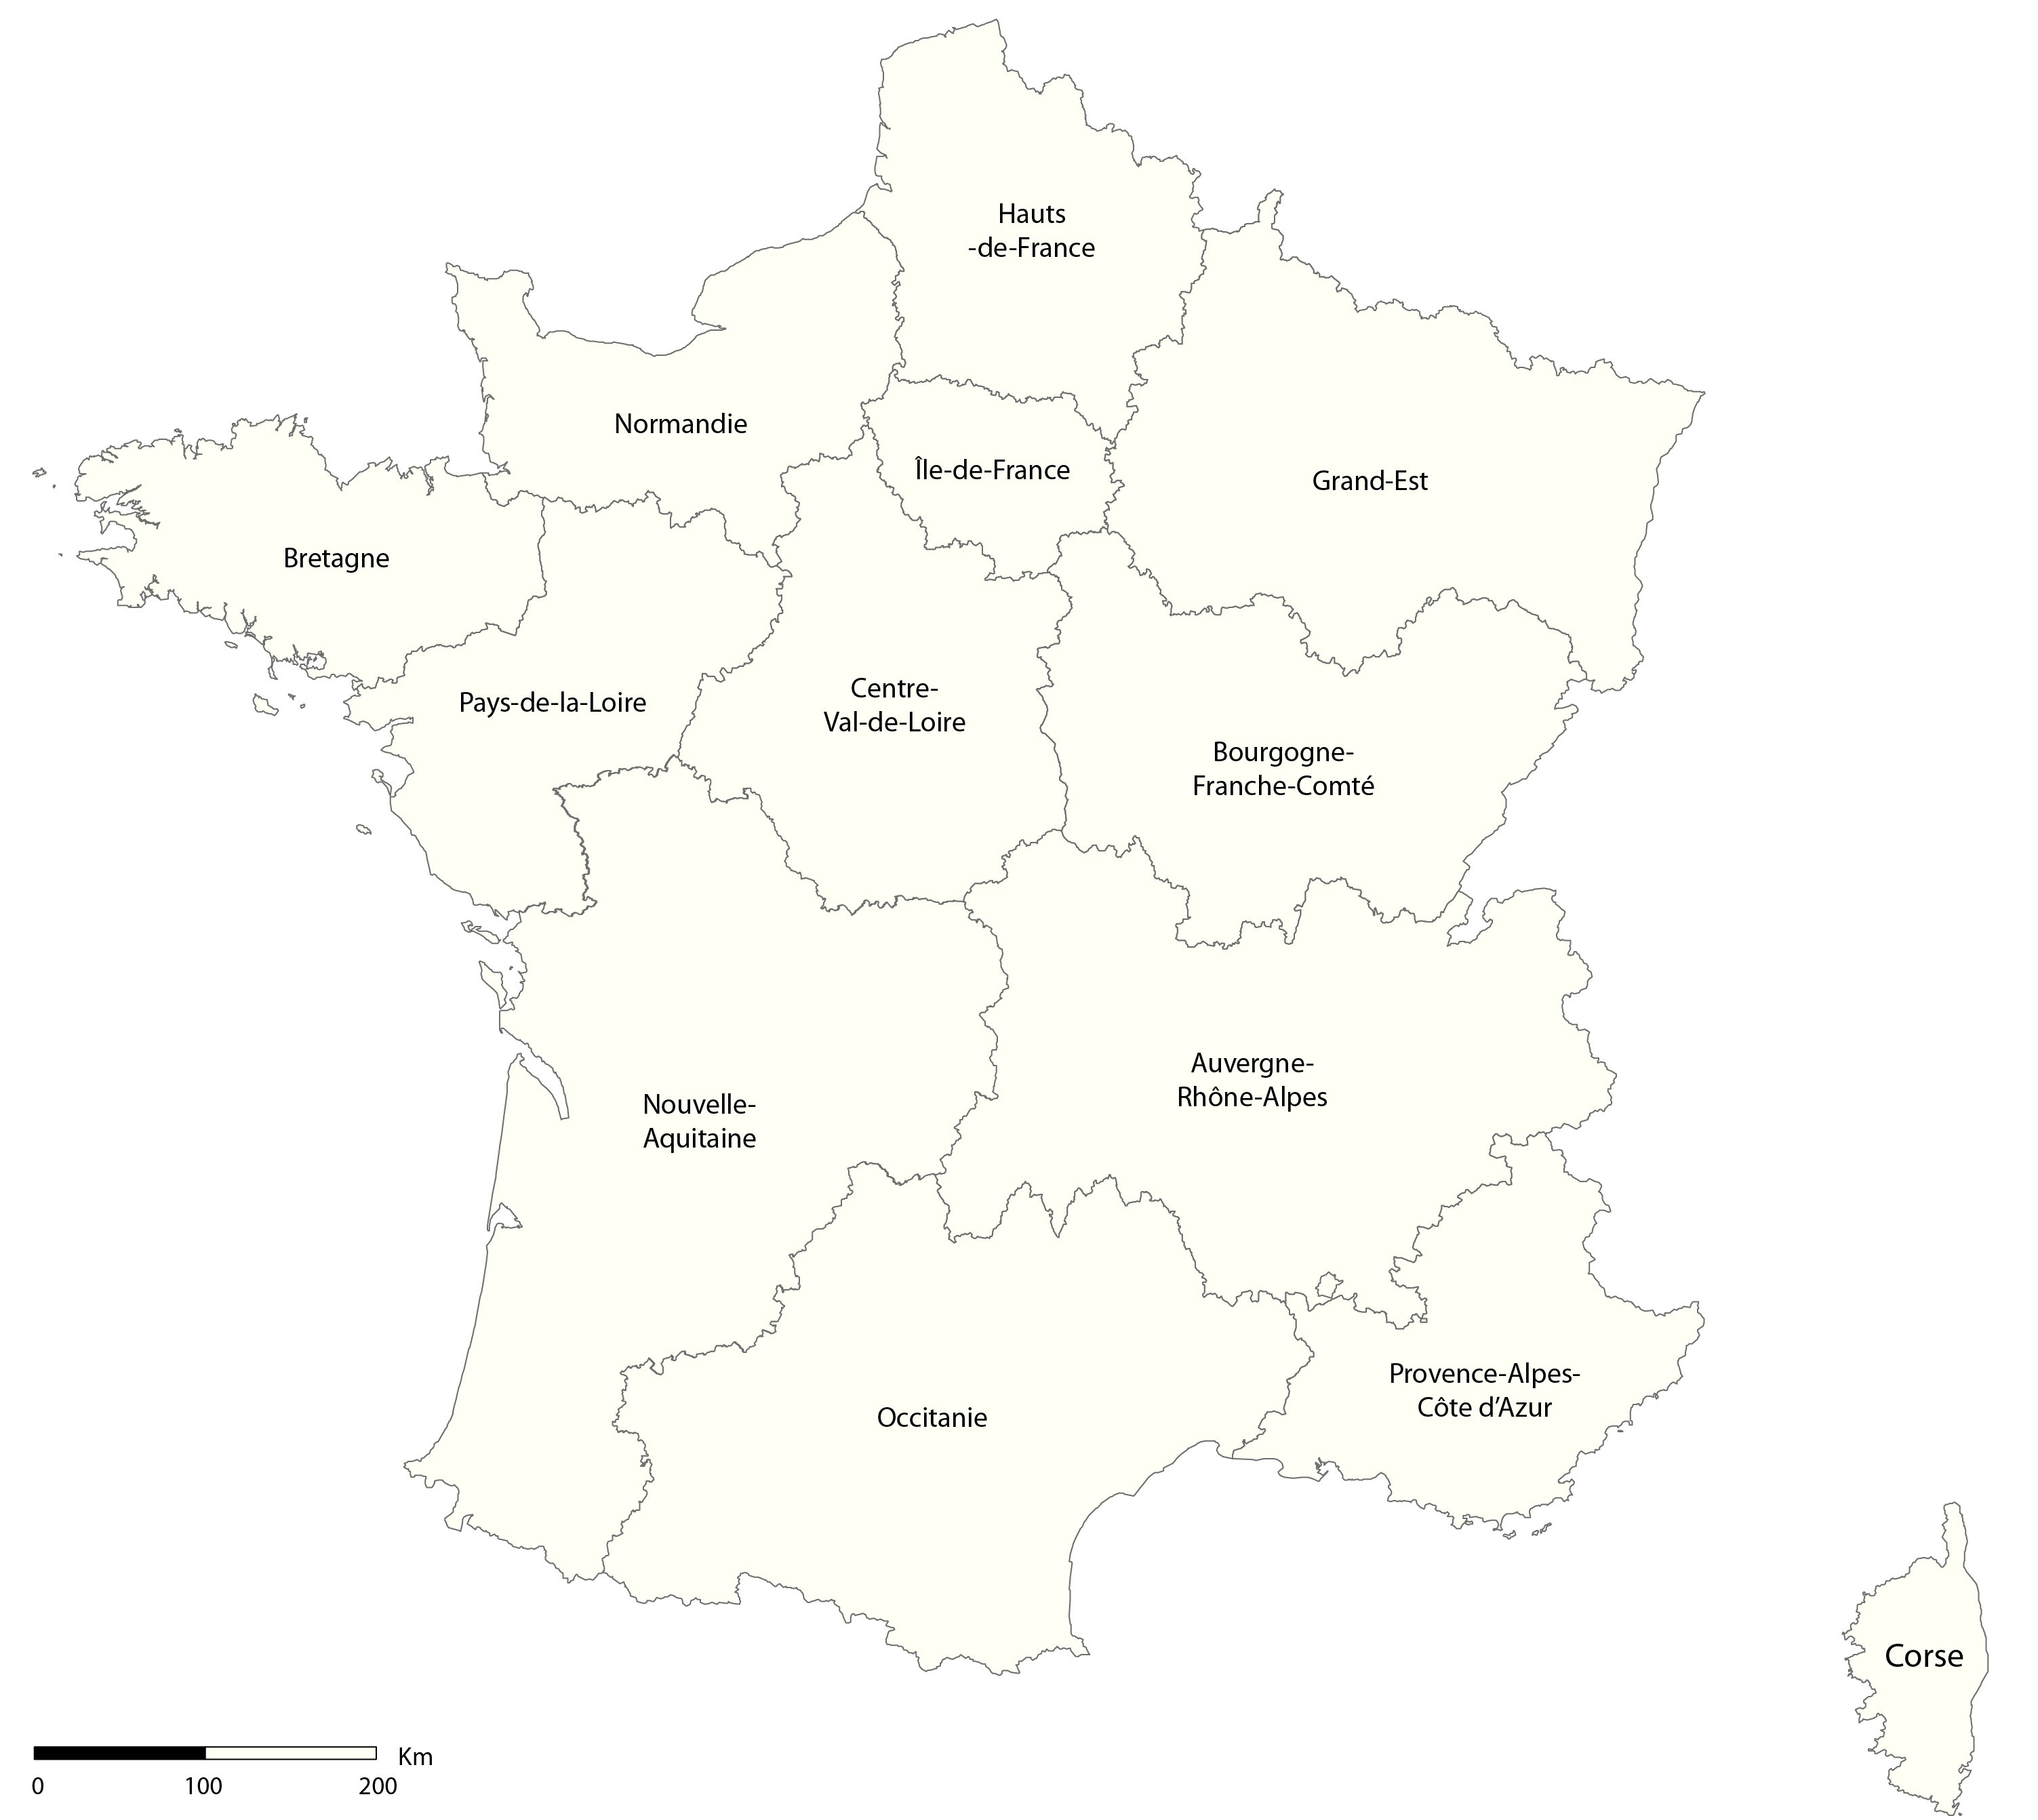
\includegraphics[width=10cm]{france-region.jpg} etex;
% picture from https://capcarto.fr/telechargements/
draw grid(20,18)(u);
defnodes((4.5u,12.5u),(7.5u,14.5u),(5u,10u),(9.5u,16.5u),(10u,13u),
          (15u,13u),(9u,12u),(12u,11u),(6u,8u),(11u,7u),(9u,3u),
          (15u,5u),(19u,1u));
nodebgcolor:=red;
drawnodes(7,4,11,13);
nodebgcolor:=green;
drawnodes(2,10,6);
nodebgcolor:=blue;
drawnodes(5,3,12);
nodebgcolor:=(1,1,0);
drawnodes(1,8,9);
drawedges((1,2),(1,3),(2,3),(2,4),(2,5),(2,7),(3,7),(3,9),(4,5),
          (4,6),(5,6),(5,7),(5,8),(6,8),(7,8),(7,9),(7,10),(8,10),
          (9,10),(9,11),(10,11),(10,12),(11,12))();
\end{exemple}



\subsection*{Markov chain}

\begin{exemple}[lefthand ratio = 0.6]
scaleprob:=0.8;
u:=1.6cm;
nodebgcolor:=0.8white;
defnodes((0,0),(2u,0),(u,1.5u));
drawnodes();
drawoptions(withcolor red);
drawdiredges((1,2),"$0.5$",(1,3),"$0.3$")(-25);
drawdiredge(1,1)("$0.2$",210);
drawoptions(withcolor blue);
drawdiredges((2,1),"$0.1$",(2,3),"$0.3$")(-25);
drawdiredge(2,2)("$0.6$",-30);
drawoptions(withcolor 0.5green);
drawdiredges((3,1),"$0.7$",(3,2),"$0.2$")(-25);
drawdiredge(3,3)("$0.1$");
\end{exemple}

\subsection*{Hypercube $Q_3$}

\begin{exemple}[lefthand ratio = 0.65]
u:=3cm;
nodewidth:=0.3cm;
edgelinewidth:=2;
pair p; p:=(0.4u,0.4u);
defnodes((0,0),(u,0),(0,u),(u,u));
defnodes((0,0)+p,(u,0)+p,(0,u)+p,(u,u)+p);
nodebgcolor:=black;nodelinecolor:=black;
drawnode.lrt(6,"101");
nodebgcolor:=red;nodelinecolor:=red;
drawnode.llft(1,"000");drawnode.lrt(2,"001");
drawnode.rt(4,"011");drawnode.lrt(5,"100");
nodebgcolor:=blue;nodelinecolor:=blue;
drawnode.lft(3,"010");drawnode.ulft(7,"110");
drawnode.urt(8,"111");
drawedges((1,3),(3,4),(2,6),(4,8),(6,8),(5,6),(5,7))();
drawedges((3,7),(7,8))() withcolor blue;
drawedges((1,2),(1,5),(2,4))() withcolor red;
\end{exemple}

\subsection*{Three utilities problem}

With  Lua\LaTeX{}, \verb|luamplib| and \verb|fontawesome5| packages.

\begin{exemple}[lefthand ratio = 0.7]
u:=1.2cm;
defnodes((u,2u),(2u,2u),(3u,2u),(u,u),(2u,u),(3u,u));
nodelinecolor:=white;
drawnode(1,"\large \faHome");
drawnode(2,"\large \faHome");
drawnode(3,"\large \faHome");
nodebgcolor:=black;nodefgcolor:=blue;
drawnode(4,"\faWater");
nodefgcolor:=red;drawnode(5,"\faBurn");
nodefgcolor:=(1,1,0);drawnode(6,"\faBolt");
drawedges((1,4),(2,4),(2,5),(2,6),(3,6))();
drawedges((1,5),(5,3))(-115);
vardef edgeshape(expr A,B)=
save a;numeric a;a=angle(B-A);s:=if A>B: - fi 1;
A..(0.7[A,B]+(0.35(B-A) rotated (s*90))){dir a}..B
enddef;
drawedges((4,3))();
edgelinewidth:=2;drawedges((6,1))() withcolor (1,0.5,0);
\end{exemple}

\subsection*{Various}

\begin{exemple}[lefthand ratio = 0.6]
nodebgcolor:=0.7white;
nodewidth:=0.2cm;

for i=1 upto 7:
  defnode(A[i],(2cm,0) rotated (360*i/7));
  drawnode[360*i/7](i);
  for j=1 upto i-1:
    drawedge(i,j)();
  endfor
endfor
\end{exemple}

\begin{exemple}[lefthand ratio = 0.6]
nodebgcolor:=0.7white;
nodewidth:=0.2cm;
printnodename:=false;

u:=0.7cm;
defnodes((3u,-3u));
drawnode(1);
for i=1 upto 4:
 for j=1 upto 4:
  defnodes((0,-2u) rotatedaround((0,-3u),90j)
                      rotated 90i);
 endfor
 defnodes((3u,-3u) rotated (90i));
 drawnodes(5i-3,5i-2,5i-1,5i,5i+1);
 drawedges((5i-4,5i-3),(5i-3,5i-2),(5i-2,5i-1),
             (5i-1,5i),(5i,5i-3),(5i-1,5i+1))();
endfor;
\end{exemple}


\begin{exemple}[listing above text,before lower=\footnotesize]
u:=1.2cm;
nodewidth:=0.4cm;
defnodes((0,0.6u),(3u,0.6u),(5u,0),(8u,0),(10u,0.6u),(13u,0.6u),(0,-0.6u),
                                            (3u,-0.6u),(10u,-0.6u),(13u,-0.6u));
nodeedgeoffset:=-0.2cm;
nodebgcolor:=0.8white;
edgelinewidth:=0.2cm;
vardef edgeshape (expr A,B)=A{dir 0}..{dir 0}B enddef;
drawedges((1,2))() withcolor red;
drawedges((5,6))() withcolor red;
drawedges((7,8))() withcolor blue;
drawedges((9,10))() withcolor blue;
endedgeshift:=0.1cm;   drawedges((2,3))() withcolor red;
endedgeshift:=-0.1cm;  drawedges((8,3))() withcolor blue;
endedgeshift:=0cm;
startedgeshift:=0.1cm; drawedges((4,5))() withcolor red;
startedgeshift:=-0.1cm;drawedges((4,9))() withcolor blue;
edgeshift:=0.1cm;      drawedges((3,4))() withcolor red;
edgeshift:=-0.1cm;     drawedges((3,4))() withcolor blue;
drawnode.bot(1,"C.H.U.");
drawnode.bot(2,"Berges de Maine");
drawnode.bot(5,"Hôtel de Ville");
drawnode.bot(6,"Foch - Maison bleue");
drawnode.bot(7,"Doutre");
drawnode.bot(8,"Place Molière");
drawnode.bot(9,"Conservatoire");
drawnode.bot(10,"Montaigne");
vardef nodeshape(expr p)=
  (halfcircle shifted (0,0.5)--
   halfcircle scaled -1 shifted (0,-0.5)--
    cycle) scaled nodewidth
enddef;
drawnode.bot(3,"Saint-Serge");
drawnode.bot(4,"Centre de Congrès");
\end{exemple}

\begin{exemple}[listing above text]
vardef nodeshape(expr p)=
% From "Drawing with Metapost" by Toby Thurston
% https://github.com/thruston/Drawing-with-Metapost/
 for i=1 upto 20:
  (0.4cm if odd(i): - else: + fi 3+ uniformdeviate 3,0) rotated (i*360/20) --
 endfor cycle
enddef;
vardef edgeshape(expr A,B)=
 save an;numeric an;an:=angle(B-A);
 A{dir (an + 60*(uniformdeviate 2-1))}..
 0.5[A,B]{dir (180+an)}..
 {dir (an + 60*(uniformdeviate 2-1))}B
enddef;
nodebgcolor:=(1,0.5,0);
nodelinecolor:=0.6red;
nodefgcolor:=0.6red;
linecolor:=0.5green;
edgelinewidth:=1.5;
defnodes((0cm,0cm),(4cm,2cm),(8cm,1cm),(5cm,-3cm));
drawnodes();
drawedges((1,2),(2,3),(3,4),(1,4))();
\end{exemple}

\end{document}
